\documentclass[10pt]{article}
\usepackage[backend=bibtex,style=numeric]{biblatex}
\usepackage{enumitem}
\usepackage{graphicx}
\usepackage{caption}
\usepackage{subcaption}
\usepackage{fullpage}

\addbibresource{refs}

\title{Extracting Application and Menu Events from UI Tutorial Videos}
\author{Daniel Seita \& Andrew Head}

\begin{document}

\maketitle

\begin{abstract}
In this project, we present two main contributions. First, we show that a standard AlexNet neural
network with minimal tweaking can accurately recognize frames belonging to a class of videos.
Second, we present a pipeline for detecting menus within a video frame sequence. We then discuss how
these two stages might be combined to enhance the process of extracting information from videos.
\end{abstract}

\section{Introduction and Motivation}

In recent years, video tutorials for learning to use software have proliferated online.  
This has attracted interest in improving users' ability to learn from them~\cite{matejka_ambient_2011,
pongnumkul_pause-and-play_2011}.  Video tutorials appear to be beneficial for
some learning tasks.  Grossman \& Fitzmaurice showed that short, 10-25 second contextually-related videos were
more effective in helping users accomplish tasks than traditional text-based
tutorials~\cite{grossman_toolclips_2010}.  

Unfortunately, navigation issues lead to misunderstandings, and users can't always keep up with the pace of instruction.
Researchers found that when provided with 2-3 minute task-oriented tutorials, users perform
better with text tutorials than videos because users cannot work at the same pace as the
video~\cite{grabler_generating_2009}. This work points to a need to better segment, index, and 
enable navigation of videos to improve users' abilities to adapt to the pace of instruction.
In our project, we investigate techniques for \emph{understanding applications and menu events in UI tutorial videos through
computer vision}, with the intent to enable new methods of segmenting, indexing and navigating tutorial videos.

We build upon past work that visually reverse engineers user interfaces (UIs).
By examining pixels, many have succeeded at reverse engineering UIs and
interactions with purely visual information, independent of underlying application knowledge.  For
instance, Sikuli~\cite{yeh_sikuli_2009} uses computer vision to identify GUI elements from screen
captures with template matching for small UI elements and voting based on invariant local
features for large elements. Prefab identifies GUI elements with GUI-specific visual features~\cite{dixon_prefab_2010}
to provide an overlay of advanced interactions on existing interfaces.  The system identifies interface
elements using two strategies: exact matches of prototype pixels, and models of the background and
pixel differences to identify foreground interface elements.

Perhaps most related, Waken~\cite{banovic_waken_2012}
contributes to this research direction by discovering cursor shapes, clicking actions, icons, tooltips and
menus, all by examining the difference between frames of UI videos.  They do this by making
assumptions about how the image of icons change during hover and press actions.  Detection of the
cursor and icons in later frames is performed by template matching.  We rely on techniques similar
to those in Waken to detect when and where menus appear in UI videos.


\section{Video Classification}\label{sec:daniel}

As a first step in the information extraction pipeline, we consider the following classification
question: given a video tutorial, what application is it about? We only allow access to the raw
frames, and not metadata such as the video title.  This is an important problem because if we know
the application type of the video tutorial, then we can deploy class-specific extraction procedures,
such as template matching tools based on (for instance) Eclipse videos. Furthermore, if a video
contains multiple applications (e.g., a Microsoft Office video might contain Excel, Powerpont, and
other related products) we might be able to segment the video based on application type, which ties
in to one of our original project goals.

\begin{figure}[t]
\centering
  \begin{minipage}{.4\textwidth}
  \centering
  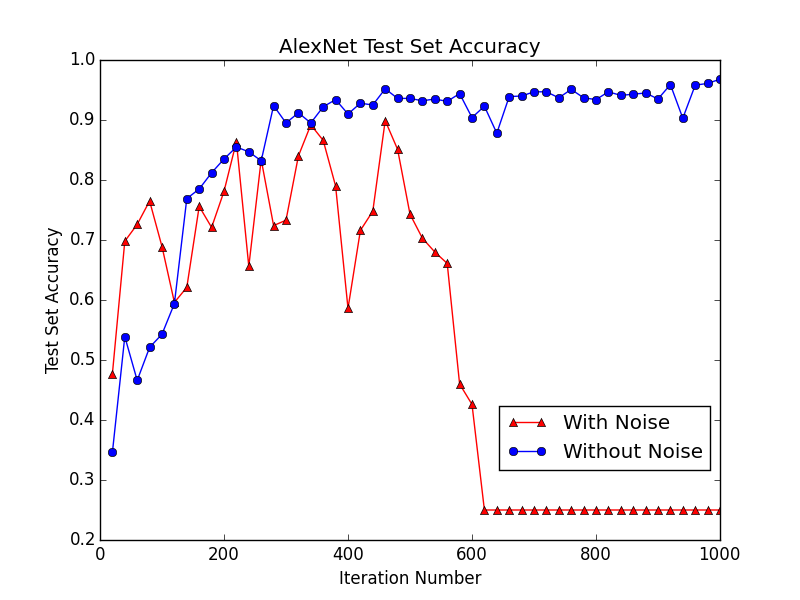
\includegraphics[width=1\linewidth]{AlexNet_Accuracy1000}
  \caption{AlexNet accuracy results of two networks trained on two image datasets.}
  \label{fig:alex_net}
  \end{minipage}\hfill
  \begin{minipage}{.4\textwidth}
  \centering
  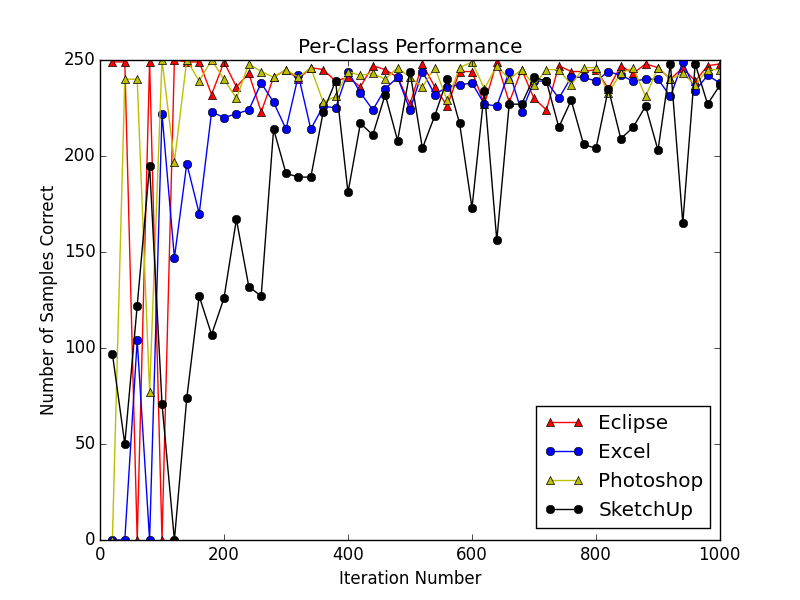
\includegraphics[width=1\linewidth]{PerClassPerformance1000}
  \caption{AlexNet per-class accuracy results for our ``noiseless'' network.}
  \label{fig:per_class}
  \end{minipage}
\end{figure}

To collect training data, we used the \texttt{youtube-dl} software to download YouTube videos into
mp4 format. We restricted our focus to videos about Eclipse, Excel, Photoshop, and SketchUp, and we
extracted from playlists to maintain consistency. Then we used the \texttt{ffmpeg} software to
extract one frame per second from each video, which resulted in a set of 110240 JPG images, roughly
evenly split among the four classes. 

We observed that many of our videos had special introductory and concluding scenes that were of a
different style than the true content of the video. Thus, we created two datasets: one with
\emph{all} the frames, and one with the \emph{first and last ten frames removed} for each video.
Since we had one frame per second, this was equivalent to ``cropping'' each video by ten seconds on
both sides. This cropped dataset, which also included cropped validation and testing frames, was
termed the ``no noise'' data. We randomly divided both datasets into training, validation, and
testing sets, with 52000 training images (13000 per class), 8000 validation images (2000 per class),
and 1000 testing images (250 per class).

To train our network, we used CAFFE's pre-provided AlexNet architecture, but increased the momentum
from 0.9 to 0.99 and decreased the base learning rate from 0.01 to 0.001. We did this because our
batch size of 32 was smaller than the standard 256, so our updates would have been noisier on
average. We ran training for 1000 iterations on both datasets and saved every 20th architecture for
testing purposes.

Figure~\ref{fig:alex_net} shows accuracy results for the two AlexNet networks we trained on the
1000-image test set. The architecture trained on all the data performed inconsistently and its
accuracy eventually leveled off at 25 percent since it always guessed that frames belonged to
SketchUp videos. In contrast, the ``noiseless'' data architecture performed very well, with accuracy
peaking at 96.1 percent after 1000 iterations.

We also investigated per-class accuracy results to see if certain classes of video frames were
harder to learn than others. Figure~\ref{fig:per_class} shows results for the ``no noise'' AlexNet
network. It is clear that SketchUp videos are initially the hardest to learn to identify;
fortunately, by the time we reach 500 iterations, our network can correctly classify the vast
majority of images across all four classes.

We then investigated the 96 filters for the first layer of the AlexNet architecture, each of which
has dimension $55\times 55$. Figures~\ref{fig:filters_all} and~\ref{fig:filters_nonoise} show
visualizations for the two architectures taken after 1000 iterations of training. There are some
interesting patterns, such as straight lines and rough, curved shapes.

\begin{figure}[t]
\centering
  \begin{minipage}{.35\textwidth}
  \centering
  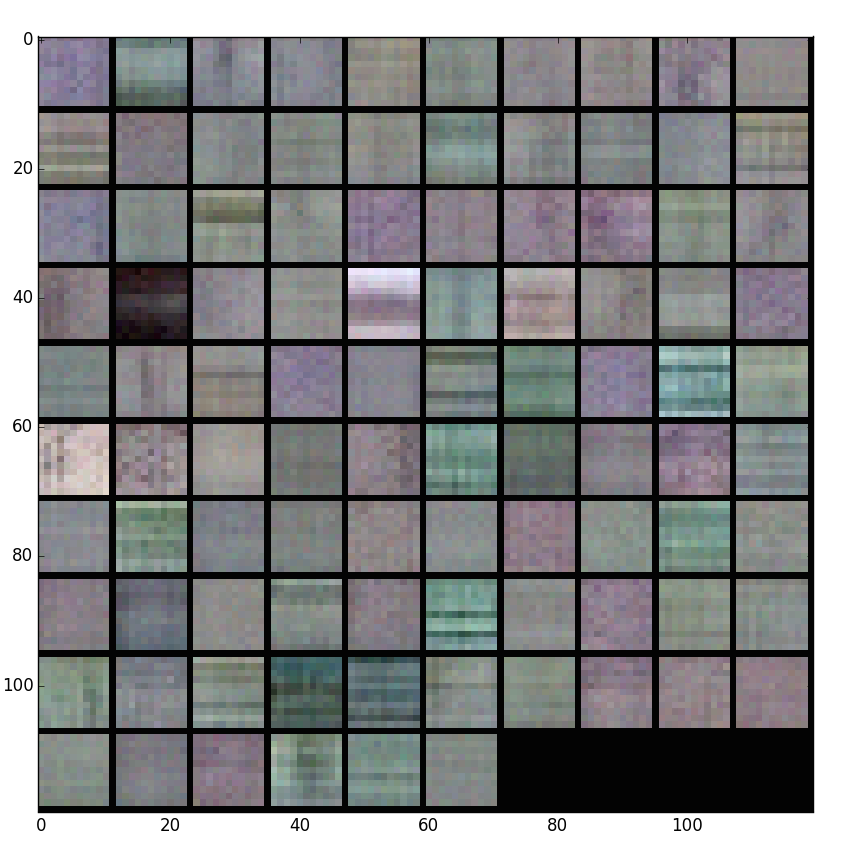
\includegraphics[width=1\linewidth]{Filters_All1000}
  \caption{Visualization of filters from the network trained on all data.}
  \label{fig:filters_all}
  \end{minipage}\hfill
  \begin{minipage}{.35\textwidth}
  \centering
  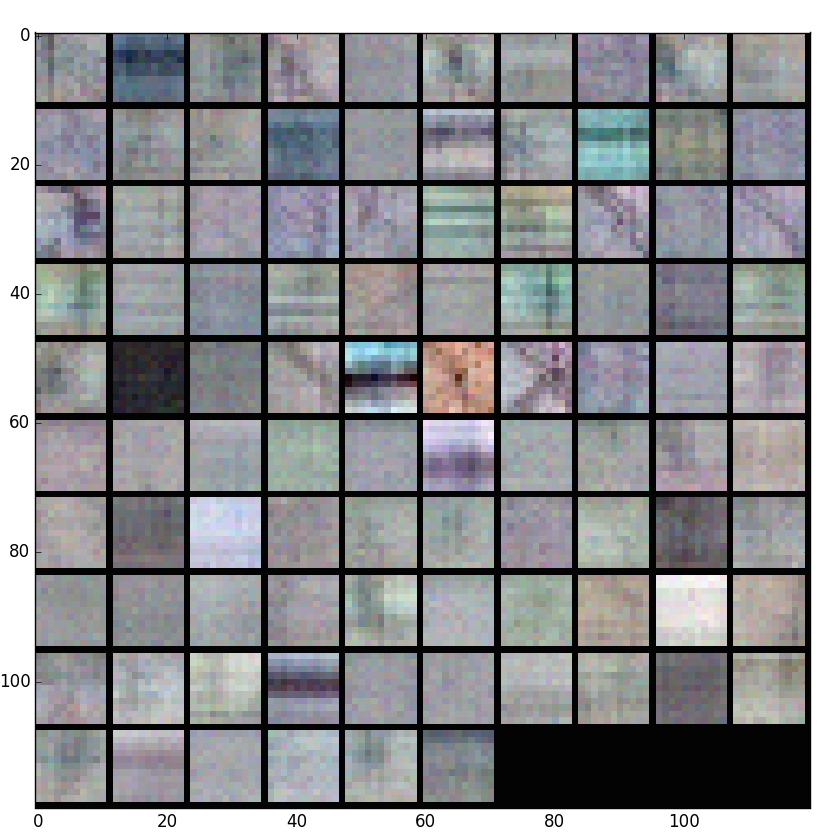
\includegraphics[width=1\linewidth]{Filters_NoNoise1000}
  \caption{Visualization of filters from the network based on ``no noise'' data.}
  \label{fig:filters_nonoise}
  \end{minipage}
\end{figure}

Finally, we performed a brief, informal experiment where we applied the (``noiseless'',
1000-iteration) neural network to videos that were not part of our training or testing data. We
chose one video for each of the four classes by searching for tutorials online; we selected the
first video we found that was between 5 and 20 minutes long and not already part of our original
data. We extracted one frame per second and deleted the first and last ten frames.

To describe the output, consider a ``split'' to be $(a,b,c,d)$, which indicates that $a, b, c,$ and
$d$ frames were classified as Eclipse, Excel, Photoshop, and SketchUp, respectively.  The Eclipse
video had $(319,0,79,0)$, the Excel video had $(610,0,71,7)$, the Photoshop had $(1,6,416,69)$, and
the SketchUp had $(9,2,233,804)$. Clearly, for the Eclipse, Photoshop, and SketchUp videos, the
classifier was able to assign the vast majority of frames to the correct class. The Excel output is
unfortunate, but intriguing because our network thought most of the frames belonged to Eclipse
videos. That video we chose was about a newer Excel version (2013) than the one we trained on
(2007).  With a wider variety of Excel frames, we would likely be able to classify that video
correctly.

\section{Locating Menus in a Frame Sequence}\label{andrew}

Recent work~\cite{banovic_waken_2012} has shown how to extract templates for cursors and icons by
monitoring pixel differences across frames of UI videos.  While there have been some initial efforts
towards recognizing tooltips and menus~\cite{banovic_waken_2012}, this task still lacks a
satisfying solution, given that reliable techniques to identify menu-based events could enable
automatic assessment of usability from UI video and provide new ways of indexing tutorial videos
based on complex user interface events.

It is challenging to detect menus based on pixel difference between frames for three reasons.  First, compressed 
video contains frame-to-frame noise that clouds the signal of a change in UI appearance, 
particularly if UI widgets tend to fade in or out gradually.  Second, when menus appear, they occlude
heterogeneous backgrounds (photos in Photoshop, colorful code in the IDE), making the difference
at each individual pixel highly-varied relative to its neighbors when a new object appears in the
foreground, even if it is of homogeneous color.  Third, depending on the operating system, 
the edges dividing menus from ribbons and borders in the main UI may be subtle compared to the
internal edges in a menu caused by text or internal horizontal lines that separate groups of options.
This makes it impossible to apply traditional segmentation techniques to extract menu regions from 
static images.

\begin{figure}
    \centering
    \begin{subfigure}{0.3\textwidth}
        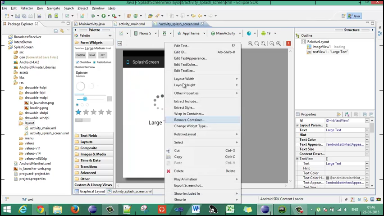
\includegraphics[width=\textwidth]{fig/pipeline1}
        \caption{}
        \label{fig:pipeline1}
        \vspace*{2mm}
    \end{subfigure}
    \begin{subfigure}{0.3\textwidth}
        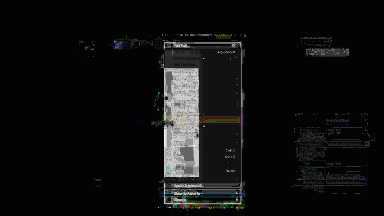
\includegraphics[width=\textwidth]{fig/pipeline2}
        \caption{}
        \label{fig:pipeline2}
        \vspace*{2mm}
    \end{subfigure}
    \begin{subfigure}{0.3\textwidth}
        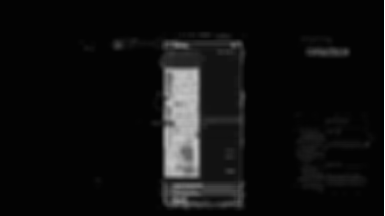
\includegraphics[width=\textwidth]{fig/pipeline3}
        \caption{}
        \label{fig:pipeline3}
        \vspace*{2mm}
    \end{subfigure}
    \begin{subfigure}{0.3\textwidth}
        
\includegraphics[width=\textwidth]{fig/pipeline4}
        \caption{}
        \label{fig:pipeline4}
    \end{subfigure}
    \begin{subfigure}{0.3\textwidth}
        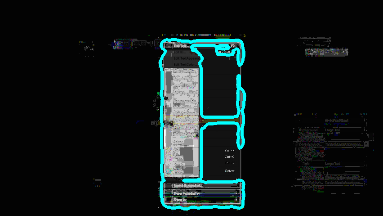
\includegraphics[width=\textwidth]{fig/pipeline5}
        \caption{}
        \label{fig:pipeline5}
    \end{subfigure}
    \begin{subfigure}{0.3\textwidth}
        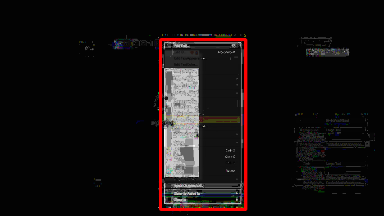
\includegraphics[width=\textwidth]{fig/pipeline6}
        \caption{}
        \label{fig:pipeline6}
    \end{subfigure}
    \caption{Our pipeline for extracting UI menu locations from a sequence of video frames.}
\end{figure}

We propose a method for extracting regions containing menus based on frame-to-frame pixel
differences.  We address the first two of the three detection challenges described above.

Our pipeline comprises three major steps.  First, we perform \emph{temporal smoothing}
of frame-to-frame pixel differences by averaging pixel differences over a window of size 10 
(Figure~\ref{fig:pipeline2}).  This reduces noise due to compression and enables us to detect
menus that fade in instead of appearing instantly.  10 frames is one-third of a second in a $29.97fps$ video, 
long enough to capture the entire fade-in of a menu in Windows 7 (3-5 frames)
and short enough to avoid capturing multiple menu actions in the same window.  Second, we \emph{coalesce
pixel differences} into a blob that spans the menu.  We perform heavy smoothing to remove
discontinuities in edge segments and bridge blobs from menu text (Figure~\ref{fig:pipeline3}).
We binarize the smoothed image at a heuristically-determined threshold (Figure~\ref{fig:pipeline4}).
Finally, we use existing methods for \emph{contour detection} to trace the blob outline (Figure~\ref{fig:pipeline5}),
from which we take a rectangular bounding box as a region proposal (Figure~\ref{fig:pipeline6}).
We ignore all blobs that are smaller than 5000 pixels (around $70x70$ pixels square) to filter
out false positives from noisy regions of the screen.

To test our technique, we found 33 menu appearance events in 5 tutorial videos about Android development
in the Eclipse IDE.  This sample covered 3 different operating systems.
For each menu appearance, we selected the first frame where the menu was fully opaque in the video
(i.e., after fade-in) and manually determined its ground truth bounding box.

The quality of our region proposals is promising.  Our technique locates region proposals that
overlap with the ground truth in 30/33 (91\%) of the test events.  We see an average 
intersection-over-union of 74\%.  Our technique produced only 2 false positive bounding rectangles 
for all menu appearances.  We note that the strength of our technique varies by
operating system.  For example, our system produced low-overlap region proposals
on a Windows 2000-style interface, where the menu and application background color were likely
indistinguishable to our difference detection methods (Figure~\ref{fig:proposal5}, Figure~\ref{fig:proposal6}).

\begin{figure}
    \centering
    \begin{subfigure}{0.15\textwidth}
        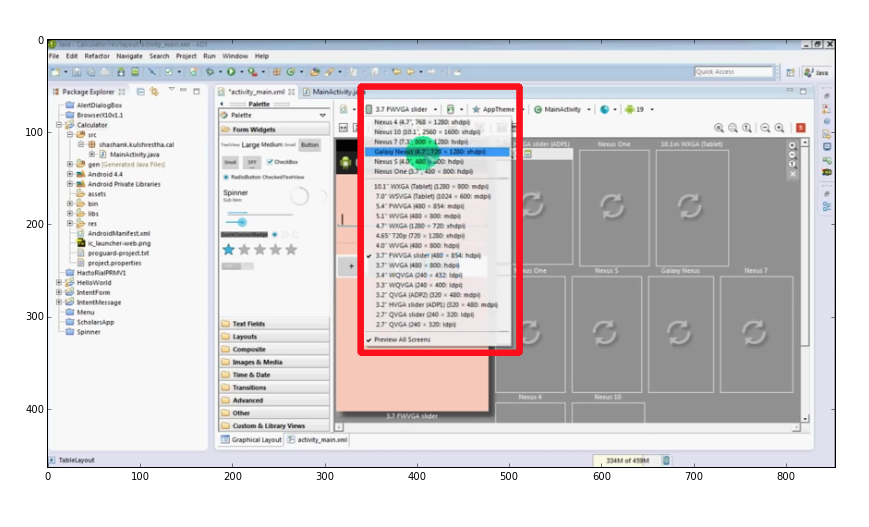
\includegraphics[width=\textwidth]{fig/proposal1}
        \caption{}
        \label{fig:proposal1}
        \vspace*{2mm}
    \end{subfigure}
    \begin{subfigure}{0.15\textwidth}
        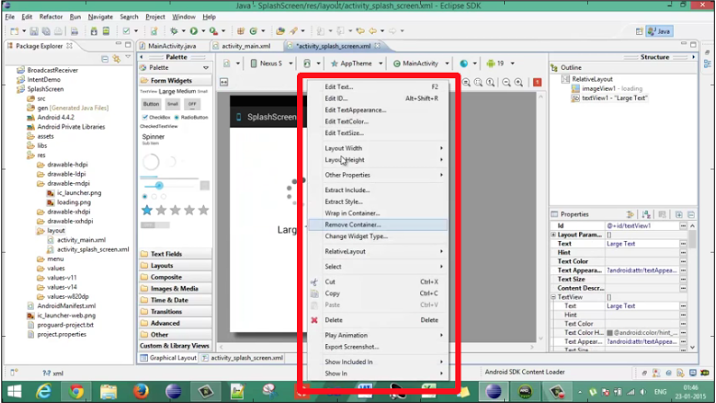
\includegraphics[width=\textwidth]{fig/proposal2}
        \caption{}
        \label{fig:proposal2}
        \vspace*{2mm}
    \end{subfigure}
    \begin{subfigure}{0.15\textwidth}
        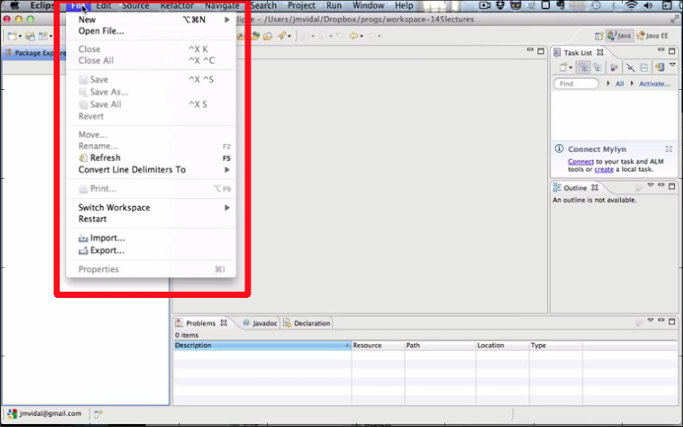
\includegraphics[width=\textwidth]{fig/proposal3}
        \caption{}
        \label{fig:proposal3}
        \vspace*{2mm}
    \end{subfigure}
    \begin{subfigure}{0.15\textwidth}
        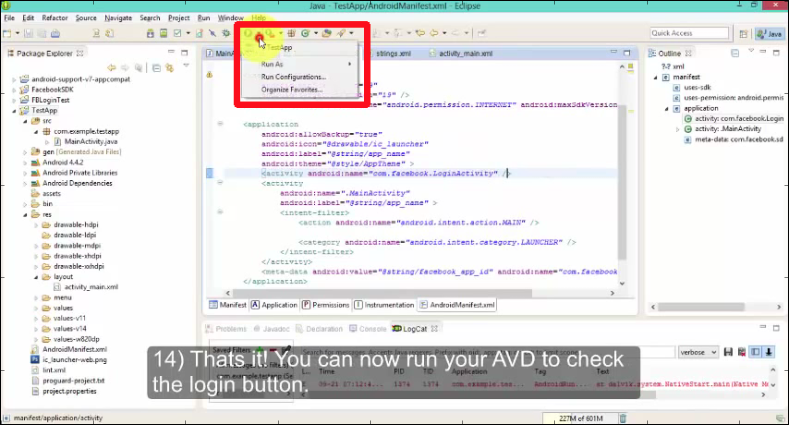
\includegraphics[width=\textwidth]{fig/proposal4}
        \caption{}
        \label{fig:proposal4}
        \vspace*{2mm}
    \end{subfigure}
    \begin{subfigure}{0.15\textwidth}
        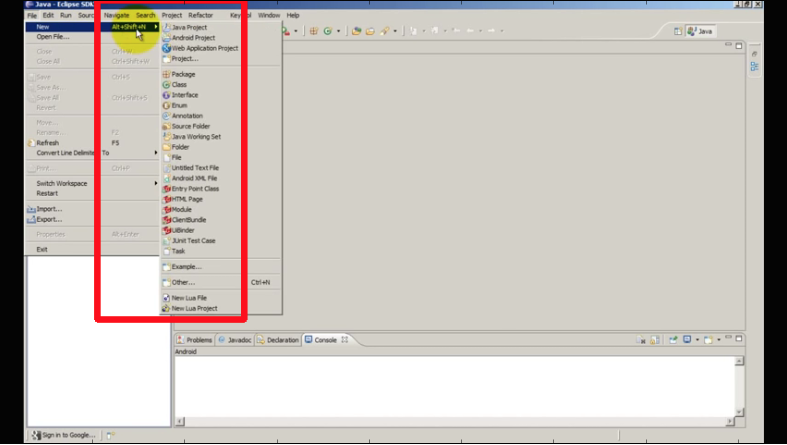
\includegraphics[width=\textwidth]{fig/proposal5}
        \caption{}
        \label{fig:proposal5}
        \vspace*{2mm}
    \end{subfigure}
    \begin{subfigure}{0.15\textwidth}
        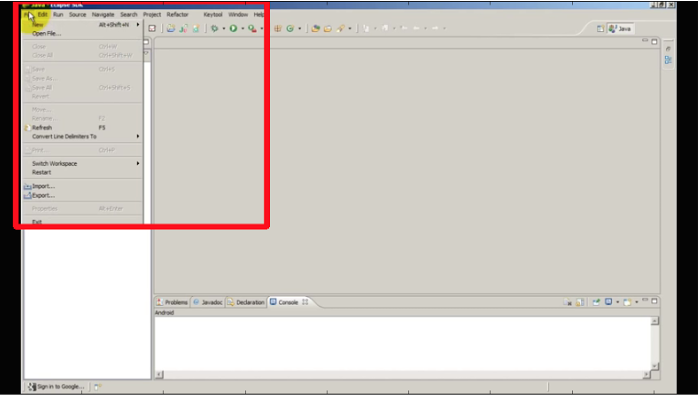
\includegraphics[width=\textwidth]{fig/proposal6}
        \caption{}
        \label{fig:proposal6}
        \vspace*{2mm}
    \end{subfigure}
\end{figure}

Our technique shows promise for extracting menu regions from UI videos.  We took preliminary efforts
to determine how to detect frame indexes where menus appear.  We hypothesize that frames with a 
high absolute pixel difference over their predecessors contained UI events.  To test this hypothesis, 
we extracted frames from one tutorial video for which the absolute pixel difference in the last 10
frames was in the 90th percentile of all differences.  Taking a sample of 50 of these frames, we confirmed that
\emph{nearly all} frames in this percentile showed a UI event in progress.  Of these, only 6 (12\%) 
were menu appearances or disappearances.  We conclude that while pixel difference-based inspection of frames may lead to
high precision detection of UI events in general, more specialized techniques are needed to
delineate menu-based UI events from application switches, window repainting, and window
appearances and disappearances in the future.

\section{Discussion and Conclusion}

We have described a classifier that can classify video frames, and a pipeline for extracting menus
from videos. Future work would ideally integrate both steps in an overall data mining pipeline by
using class knowledge to develop more specific templates for menu extraction.

\printbibliography

\end{document}
